\documentclass[10pt,a4paper]{article}
\usepackage[utf8]{inputenc}
\usepackage{amsmath}
\usepackage{amsfonts}
\usepackage{amssymb}
\usepackage{graphicx}
\usepackage[left=2cm,right=2cm,top=2cm,bottom=2cm]{geometry}
\usepackage{matlab-prettifier}
\title{Exploring Support Vectors Machines and Least Squares Support Vector Machines}
\author{Boris Shilov}

\begin{document}
\maketitle
\section{Exercise I: Basic support vector machines}
\section{Exercise II: Function estimation and time series prediction}

In this exercise I will attempt to explore the least squares support vector machine formulation using the LS-SVM Matlab toolbox \cite{pelckmansLSSVMlabMATLABToolbox}, particularly function estimation and time series prediction. 

Least-squares support vector machine is an extension of the support vector machine approach in which the quadratic problem of the classic SVM formulation is replaced by the problem of solving a set of linear equations, which is more tractable, giving a large improvement in performance. A drawback presents itself in the fact that LS-SVM requires all of the training points to be used, and hence the solution is no longer sparse, unlike the classic approach where one need only preserve a few support vectors. LS-SVM uses a least squares cost function, as the name implies, but also uses equality constraints, unlike SVM \cite{valyonRobustLSSVMRegression2007}. The function to be minimised over the set of weights (or normals) $w$, the bias term $b$ and the $e$ error to find a solution in LS-SVM is:
$$
J_p(\mathbf{w}, e) = \frac{1}{2}\mathbf{w}^T\mathbf{w} + C \frac{1}{2} \sum^N_{i=1}{e^2_i}
$$

With equality constraints $d_i = \mathbf{w}^T\varphi(\mathbf{x_i}) + b + e_i$, where $\varphi$ is some function that maps $\mathbf{x_i}$ into a higher dimensional feature space.

We can vary $e$ and also the $C$ penalty parameter, increasing which places more weight on $e$ variables.

\subsection{Support vector machine for function estimation}
Using the \texttt{uiregress} graphical command, we can construct toy datasets. 

First, let us create a dataset where a linear classifier is optimal. One such example is a close cloud of points that are intended to have come from a straight line, which we construct to have 43 points. Increasing $e$ above $0.25$ leaves no support vectors, under that the number of support vectors goes up to the number of training points, when $C$ is held fixed at infinity. Decreasing $C$ leads the line to align with the principal direction of the cloud. Setting $C=0.5$ and $e=0.1$ leads to a good fit, shown in \ref{fig:uiregress}. Noticeably, the sparsity property comes into play here. By setting the $e$ parameter above zero, we ignore errors smaller than this value. Hence, we only use a subset of the training points, achieving a measure of sparseness. This is similar to the $\epsilon$-insensitive loss function in standard SVM \cite{valyonRobustLSSVMRegression2007}.

\begin{figure}[h!]
\centering
  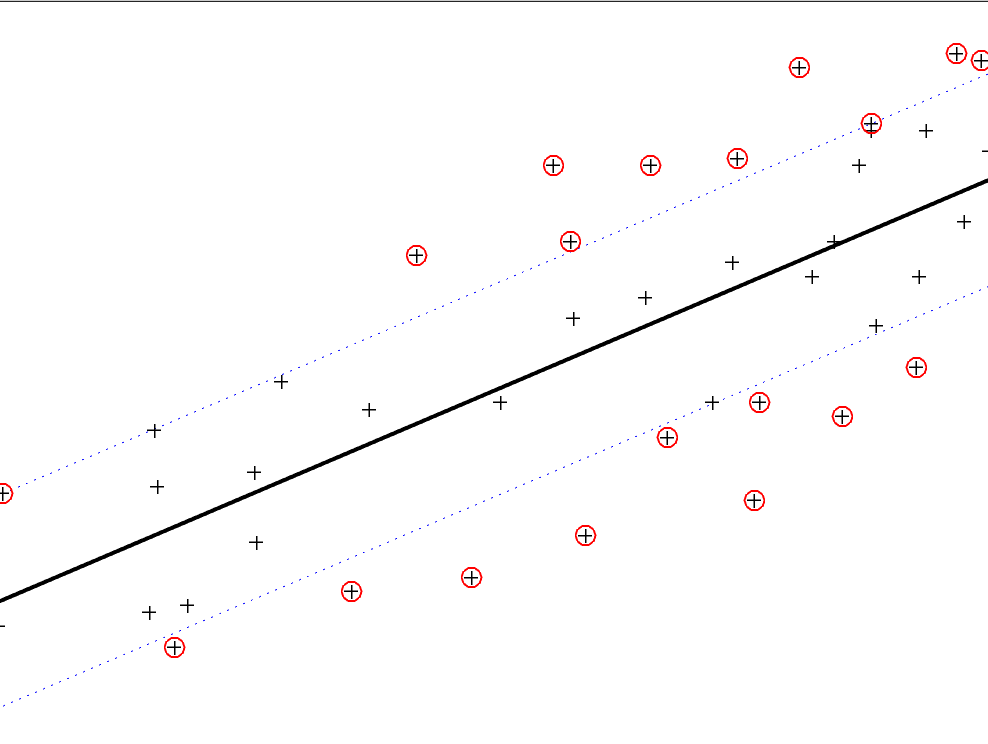
\includegraphics[width=3in]{uiregressFinal.png}
  \caption{A linear least squares regression fitted to a data cloud of 43 points with parameters $C=0.5$ and $e=0.1$. Given these parameters, only 23 points are used as support vectors, labelled in red.}
  \label{fig:uiregress}
\end{figure}

A more challenging toy dataset is one that a linear kernel cannot approximate well. Let us construct one with 46 points that is wave-like. Here, a polynomial kerne of third degree, with $C=3$ and $e=0.06$, fits quite well with quite some sparsity.

\begin{figure}[h!]
\centering
  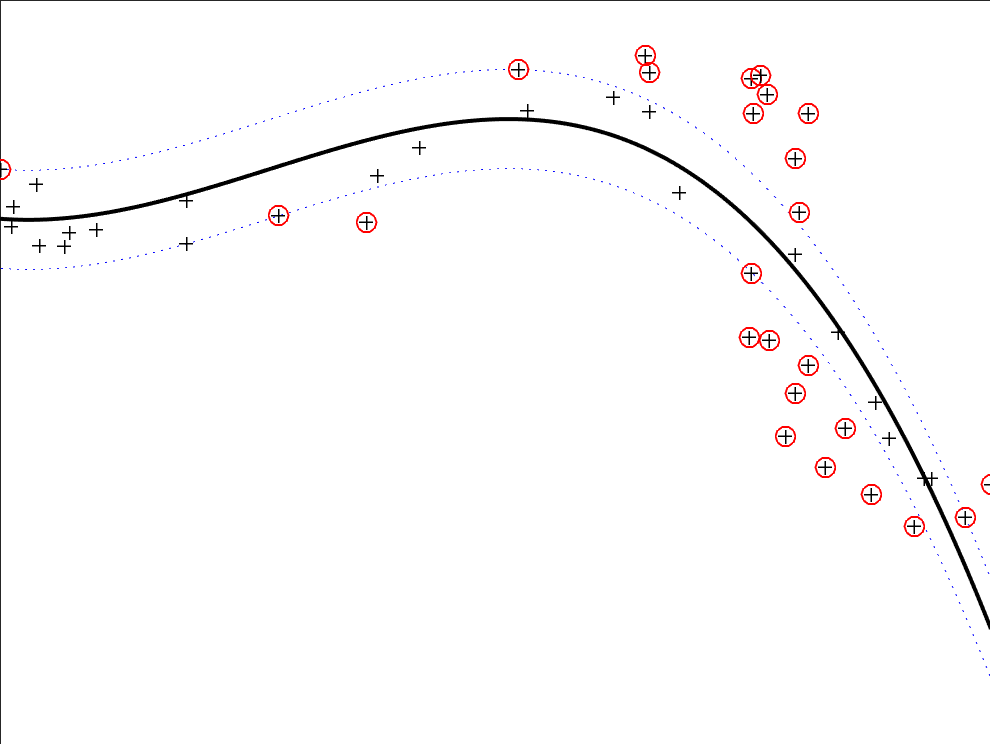
\includegraphics[width=3in]{uiregressPoly.png}
  \caption{A third degree polynomial least squares regression fitted to a data wave of 46 points with parameters $C=3$ and $e=0.06$. Given these parameters, only 26 points are used as support vectors, labelled in red.}
  \label{fig:uiregressPoly}
\end{figure}

The relation between least-squares SVM and ordinary least squares is straightforward. Both are types of regression analysis (or, at least, LS-SVM can be used as such), and use the least squares method for solving their respective systems of equations, where the sum of the squared differences between the actual datum and the prediction at the corresponding datum made by the model is minimised. In the case of OLS, linear models are used, whereas we use the SVM formulation for LS-SVM. This leads to, for example, a different definition of how the sum of squared differences (residuals) is calculated, with the following form in the OLS case for one residual:
$$
e_i = y_i - x_i^T b
$$

Contrast with the LS-SVM formulation of a residual:

$$
e_i = y_i - (w^T\varphi(x_i) + b)
$$

A yet larger difference between these is that OLS does not have hyperparameters, unlike LS-SVM. OLS derives all of its parameters from the training data, at least in the standard formulation with no shrinkage and such factors. LS-SVM on the other hand always requires some values of $C$ and $e$ (also known as $\zeta$) to be provided. Thus, regularisation is built into the standard formulation of LS-SVM through these hyperparameters, it does not have to be extended to implement it like OLS. This makes it easier to avoid overfitting, but introduces the issue of hyperparameter choice.

\subsection{Sinc function}

We can construct an example dataset using a noisy sinc function. Sinc is thus the true data generating process, and the task of an LS-SVM classifier will be to approximate this function without overfitting to replicate the noise.

$$
\mathbf{y} = sinc(\mathbf{x}) + 0.1 * \mathbf{z}
$$

Where each $z_i \leftarrow N(\mu, \sigma)$.

We can attempt approximation using the RBF kernel, iterating over a small parameter space of the RBF parameters, that is, values of $\gamma$ (confusingly, also referred to as $\sigma$) and $C$ (strictly speaking not an actual kernel parameter since it comes from the LS-SVM formulation).

\begin{lstlisting}[style=Matlab-editor, frame=single]
gams = [10, 10e3, 10e6]; sigmas = [0.01, 1, 100];
[sigmasMesh, gamsMesh] = meshgrid(sigmas, gams);
parameterSpace = num2cell([gamsMesh(:), sigmasMesh(:)], 2);
\end{lstlisting}

We can then evaluate model performance for each combination of these parameters.

\begin{lstlisting}[style=Matlab-editor, frame=single]
perfList = cellfun(@(cell) crossvalidate({ Xtrain , Ytrain , 'f', ...
    cell(:, 1), cell(:, 2), 'RBF_kernel'}, 10, 'mse'), parameterSpace);
\end{lstlisting}

A plot of this resulting performance is provided in Fig.~\ref{fig:crossvalidatedRBFSinc}.

\begin{figure}[h!]
\centering
  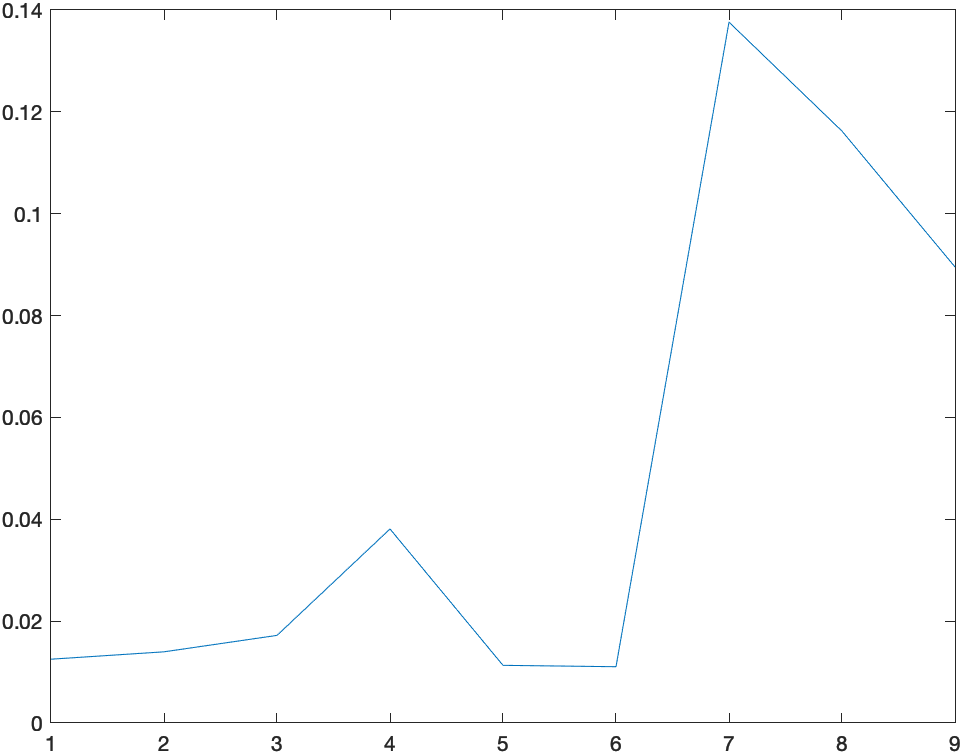
\includegraphics[width=3in]{crossvalidatedRBFSinc.png}
  \caption{A plot of LS-SVM RBF kernel predictor performance over a range of parameters.}
  \label{fig:crossvalidatedRBFSinc}
\end{figure}

It seems that the fifth and sixth models are the best fitting on training set. Their parameters are $\gamma=10000$, $c=1$ and $\gamma=10000000$, $c=1$, respectively.

We can choose between them, as well as the first two models which are relatively well fitting, using the AUC of test set performance.

\begin{lstlisting}[style=Matlab-editor, frame=single]
niceParams = cellfun(@(index) parameterSpace{index}, {1 2 5 6}, 'UniformOutput', false);
niceModelSpecs = cellfun(@(cell) { Xtrain , Ytrain , 'f', ...
    cell(:, 1), cell(:, 2), 'RBF_kernel'}, niceParams, 'UniformOutput', false);
niceModels = cellfun(@(cell) trainlssvm(cell), niceModelSpecs, 'UniformOutput', false);
niceSpecAndModel = cellfun(@(index) {niceModelSpecs{index}, ...
    niceModels{index}}, {1 2 3 4}, 'UniformOutput', false);
[Yest, Zt] = cellfun(@(cell) simlssvm(cell{1}, ...
    {cell{2}.alpha, cell{2}.b}, Xtest), niceSpecAndModel, 'UniformOutput', false);
test_mses = cellfun(@(cell) immse(cell, Ytest), Yest);
\end{lstlisting}

A plot of the test set performance shown in Fig.~\ref{fig:RBFtestsetPerf} reveals that the fifth model has the best performance.

\begin{figure}[h!]
\centering
  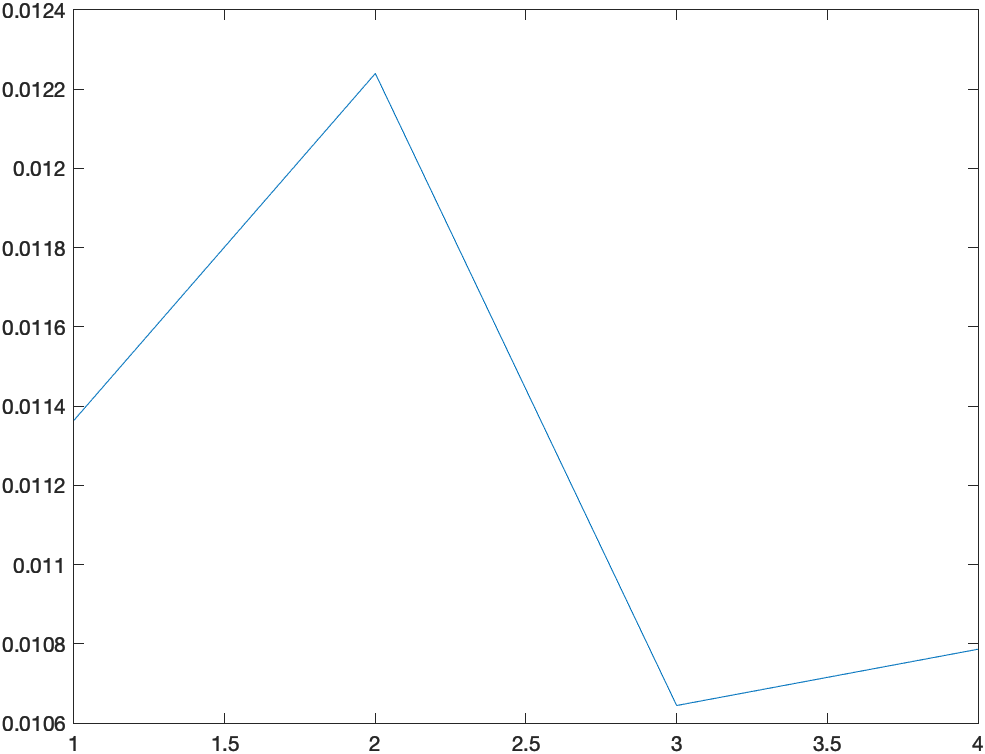
\includegraphics[width=3in]{RBFtestsetPerf.png}
  \caption{A plot of LS-SVM RBF kernel predictor performance over a range of parameters, on the test set.}
  \label{fig:RBFtestsetPerf}
\end{figure}

It seems the fifth model fits the best on the test case. We may visualise the fifth model on the test data points., shown in Fig.~\ref{fig:fifthModelPlot}. Here the hollow points are the test set that was not used to fit the data.

\begin{figure}[h!]
\centering
  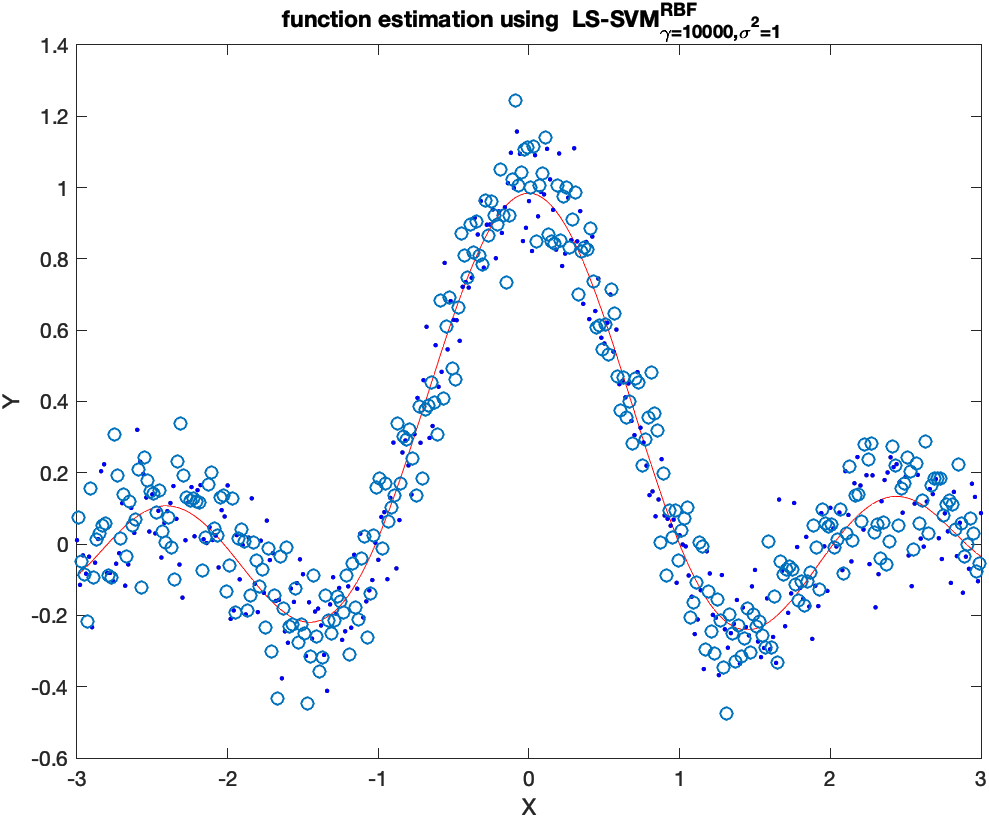
\includegraphics[width=3in]{fifthModelPlot.png}
  \caption{A plot of LS-SVM RBF kernel predictor number five out of all evaluated.}
  \label{fig:fifthModelPlot}
\end{figure}

Since the RBF kernel function estimation SVM is quite flexible, there should exist a pair of parameters that are optimal in the sense that, given these parameters, the resulting SVM is the best approximation of the underlying data-generating function possible. However, as we typically do not know directly the data generating process, a broader optimality criterion for parameters is that the resulting SVM is the best performing on some test set among the set of all possible SVMs. Some exceptions to this are possible - for example, there may be multiple near equal maxima or minima in the parameter space. This would correspond to having two or more models that fit the data equally well.

We can compare the resulting model to automatic parameter tuning.

\begin{lstlisting}[style=Matlab-editor, frame=single]
[gamSimp, sigSimp, costSimp] = tunelssvm({Xtrain, Ytrain, 'f', ...
    [], [], 'RBF_kernel'}, 'simplex', 'crossvalidatelssvm', {10, 'mse'});
 [gamGrid, sigGrid, costGrid] = tunelssvm({Xtrain, Ytrain, 'f', ...
    [], [], 'RBF_kernel'}, 'gridsearch', 'crossvalidatelssvm', {10, 'mse'});
\end{lstlisting}

The simplex procedure results in $\gamma=12727$ and $C=0.7539$. The gridsearch procedure results in parameters $\gamma=6212$ and $C=0.6857$. The cost of both is approximately the same at $0.0108$. Thus it appears we have found a better model while not using automatic parameter tuning.

\subsection{Bayesian tuning}
What is the probability that our data were generated by a particular model? How can we compare models and do regularisation using prior known information? These questions can be answered using Bayesian model comparison methodology. This process follows the principle of maximum parsimony - among all models/parameters/hyperparameters that fit well, choose the simplest \cite{MacKay91bayesianinterpolation}.

The Bayesian inference process thus provides a full framework to select models, using two levels. First, model fitting is conducted on a single mode, and we infer the most likely parameters via the posterior probability of the parameter vector. In general:
$$
P(\mathbf{w} | D, H_i) = \frac{P(D | \mathbf{w}, H_i)P(\mathbf{w} | H_i)}{P(D | H_i)}
$$
Where $\mathbf{w}$ is the parameter vector, $D$ is some data and $H_i$ is some model (\textit{hypothesis}). The denominator is the \textit{model evidence}, and since at this first stage the task is to find the most plausible parameters, it is ignored as it does not include the parameter term. The left hand side term is the posterior probability of the particular parameters $\mathbf{w}$. Thus we can pick the best parameters for a given model and data.

Once we obtain some good models, we would like to infer which model is the most probable given the data. This is the task of the second level of inference, where we defined the posterior probability of each model:
$$
P(H_i | D) \propto P(D | H_i)P(H_i)
$$
The model evidence term $P(D | H_i)$ which we previously dismissed in the first level of inference becomes important. This equation allows us to rank models using their evidence. Further, models with more parameters and thus more complexity are mathematically penalised using the so called Ockham factor (Ockham's razor is another name for the principle of maximum parsimony) \cite{MacKay91bayesianinterpolation}.

This two-step methodology is further extended for regression problems into a three-step methodology. The first step remains the same with parameter inference, but the second step is split further into a hyperparameter inference step and the model comparison step which also includes kernel parameter inference for the case of models using kernel functions such as LS-SVMs. Importantly, the hyperparameter evidence from the second step here is used in the third step. 

We can do this:

\begin{lstlisting}[style=Matlab-editor, frame=single]
sig = 0.4; gam = 10;
modelSpecBay = {Xtrain, Ytrain, 'f', gam, sig}
crit_Ls = arrayfun(@(level) bay_lssvm(modelSpecBay, level), [1 2 3])
bayOptims = arrayfun(@(level) bay_optimize(modelSpecBay, level), [1 2 3], 'UniformOutput', false);
\end{lstlisting}

The above commands perform this three step process for us. This allows us to obtain a most probable model and error bars to reflect our uncertainty.

\begin{lstlisting}[style=Matlab-editor]
sigErrs = bay_errorbar({Xtrain, Ytrain, 'f', bayOptims{2}.gam, bayOptims{3}.kernel_pars}, 'figure')
\end{lstlisting}

The model is shown in Fig.~\ref{fig:bayesianErrorbars}.

\begin{figure}[h!]
\centering
  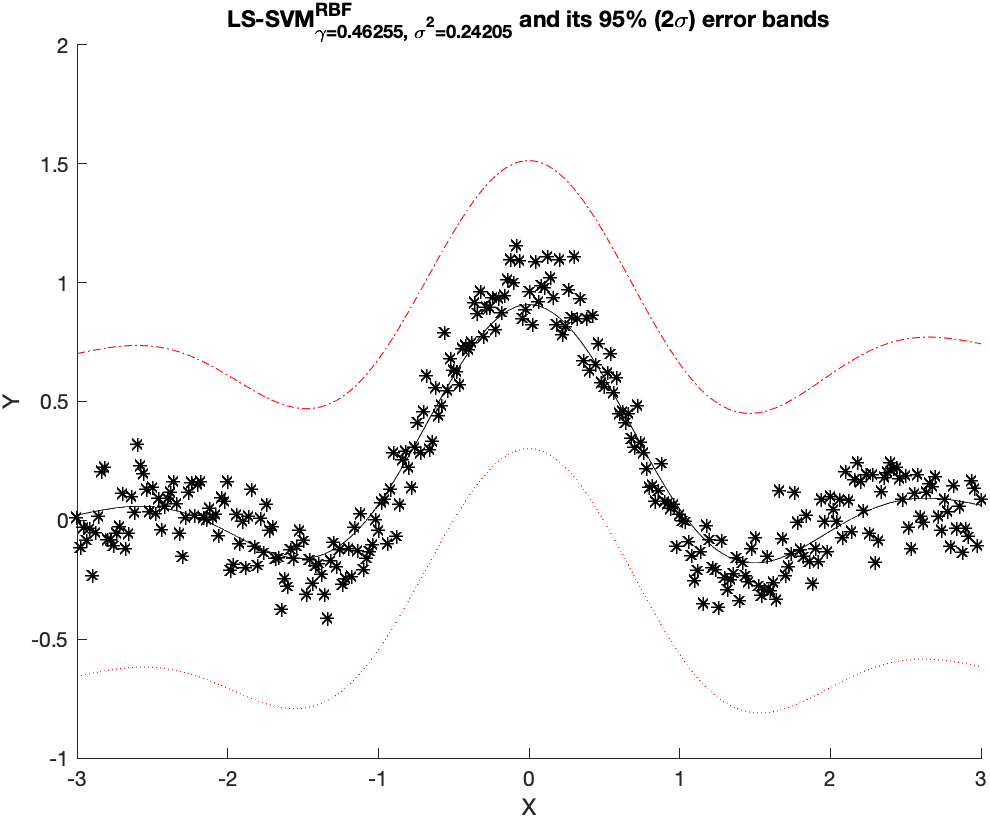
\includegraphics[width=3in]{bayesianErrorbars.png}
  \caption{The most probable model derived using Bayesian inference, with computed error bars.}
  \label{fig:bayesianErrorbars}
\end{figure}

\subsection{Automatic Relevance Determination}
Bayesian inference can further be used to remove irrelevant features and obtain a sparser subset of explanatory features. This weighs each feature (dimension) of the input space and optimises the weights at the third level of Bayesian inference.

\begin{lstlisting}[style=Matlab-editor, frame=single]
X = 6.* rand(100 , 3) - 3;
Y = sinc (X(: ,1)) + 0.1.* randn(100 ,1);
[selected, ranking] = bay_lssvmARD ({X, Y,'f', bayOptims{2}.gam, bayOptims{3}.kernel_pars});
\end{lstlisting}

Selected here are $1$ and $2$ and the ranking is $1, 2, 3$. This means that the first two dimensions of the input space are the most important, and the ranking of importance confirms this, with the third dimension being the least important.

This procedure has been shown to be equivalent to doing maximum a posteriori estimation, so an equivalent approach to this is possible using the \texttt{crossvalidate} function \cite{wipfNewViewAutomatic}.

\subsection{Robust regression}
If the data are noisy, robust regression can be used to attempt to disregard the noise and/or outliers to fit closer to the underlying function. We construct a similar sinc dataset to demonstrate this, this time adding more noise.

\begin{lstlisting}[style=Matlab-editor, frame=single]
dataGeneratingFun = @(X) sinc(X) + 0.1 * rand(size(X));
X = transpose(-6:0.2:6); Y = dataGeneratingFun(X);
outSet1 = [15 17 19]; outSet2 = [41 44 46];
Y(outSet1) = 0.7 * 0.3 + rand(size(outSet1)); Y(outSet2) = 1.5 * 0.2 + rand(size(outSet2)); 
\end{lstlisting}

The resulting dataset is shown in Fig.~\ref{fig:noisyData}.

\begin{figure}[h!]
\centering
  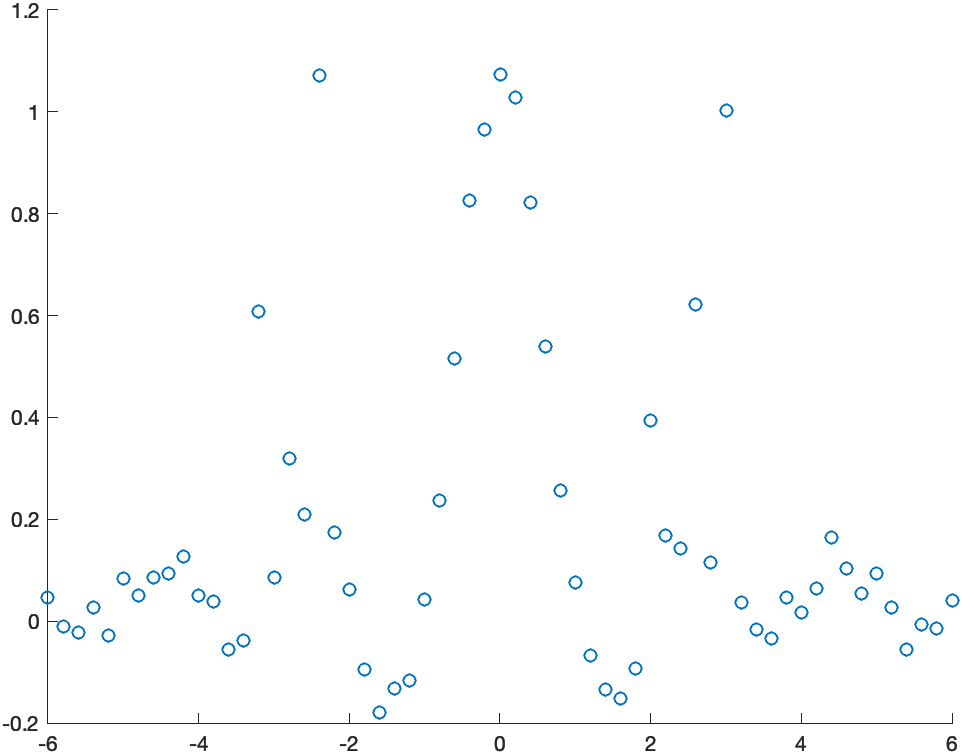
\includegraphics[width=3in]{noisyData.png}
  \caption{A noisy sinc dataset.}
  \label{fig:noisyData}
\end{figure}

What happens if we try naively fitting on these data? Fig.~\ref{fig:naiveNonRob} demonstrates.

\begin{lstlisting}[style=Matlab-editor, frame=single]
Model = initlssvm(X, Y, 'f', [], [],'RBF_kernel');
tunedNaiveModel = tunelssvm(Model, 'simplex', ...
    'crossvalidatelssvm', {10, 'mse'});
\end{lstlisting}

\begin{figure}[h!]
\centering
  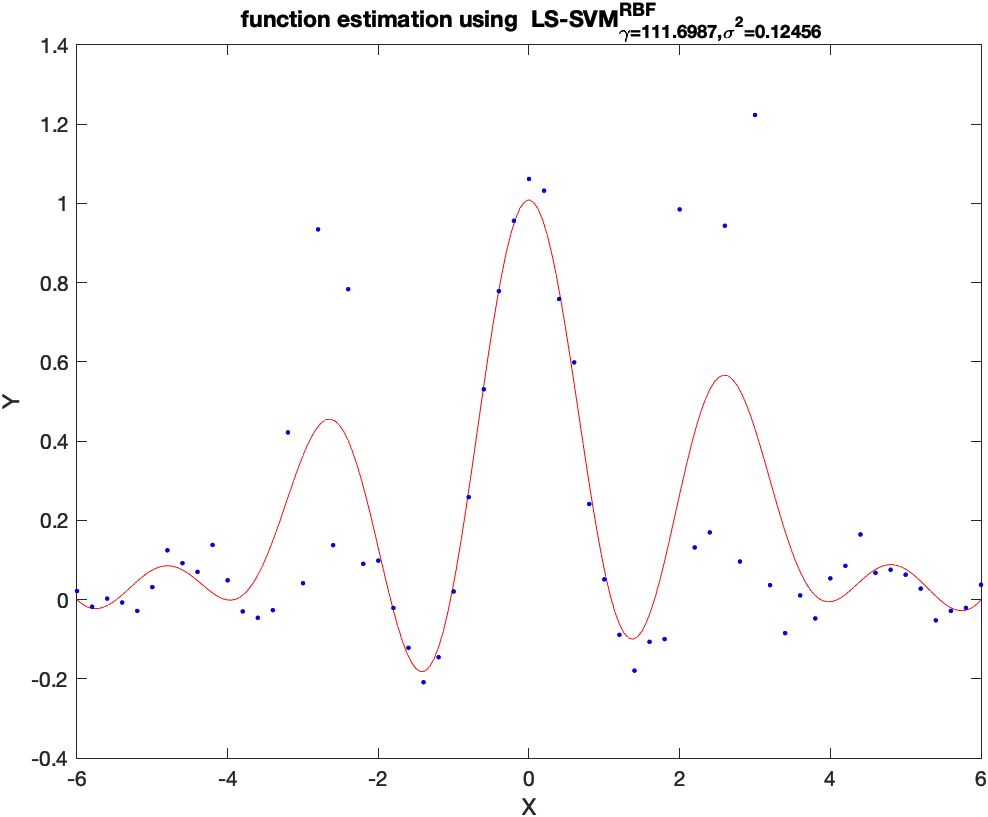
\includegraphics[width=3in]{naiveNonRob.png}
  \caption{The result of fitting a non-robust LS-SVM model to the noisy sinc data.}
  \label{fig:naiveNonRob}
\end{figure}


Within the outlier regions, the estimation is very far from the true sinc function, being highly influenced by just three points in each region. This also has effects outside the outlier regions. 
By contrast, a robust model should minimize the influence of support vectors with big errors on the final function estimate. A robust Huber's weights function model on this data will generate warning about a lack of inverse but will nonetheless produce a fit. As can be seen in Fig.~\ref{fig:whuberRobust}, this is very satisfactory and practically ignores the outliers.

\begin{figure}[h!]
\centering
  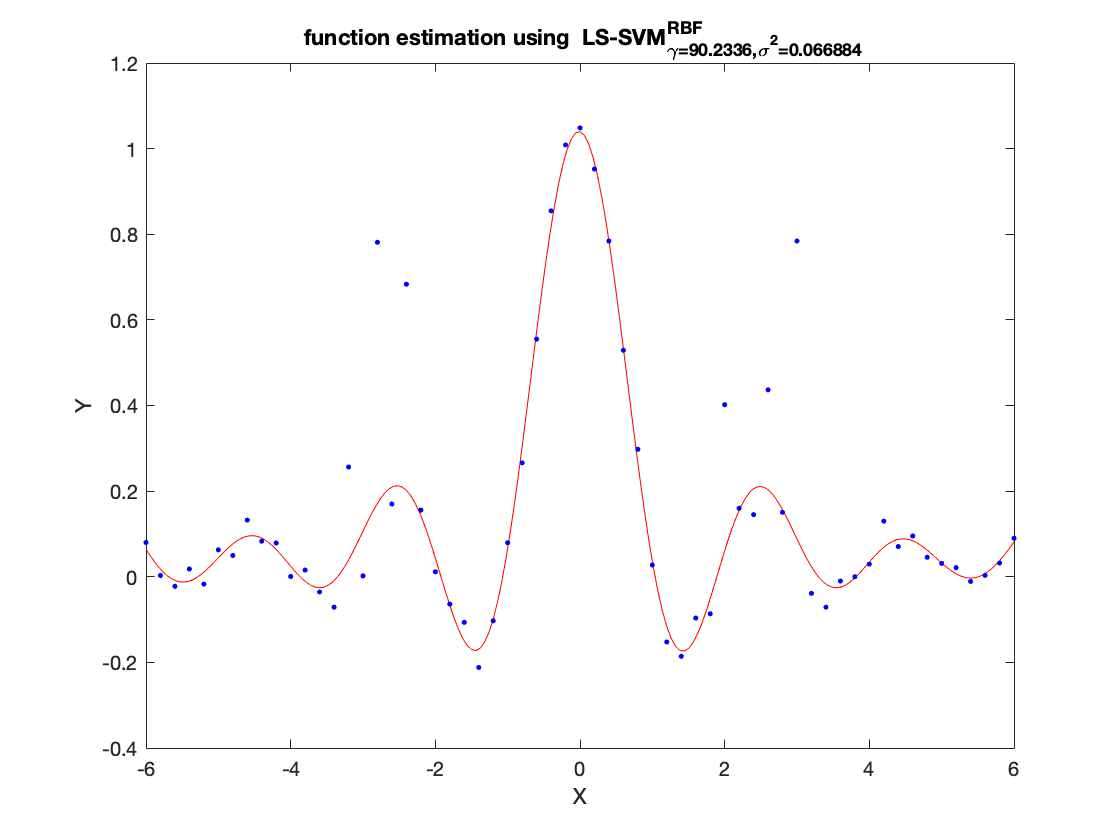
\includegraphics[width=3in]{whuberRobust.png}
  \caption{An LS-SVM regression with a Huber robust loss function on the noisy sinc data.}
  \label{fig:whuberRobust}
\end{figure}

Here the MSE function is used in the naive formulation - since the RMSE will square the residuals before summing them, this amplifies the influence of outliers. By contrast, MAE used in the robust regression penalizes large errors.

Other weight functions produce varying results. Hamper weights leads to a good approximation of the underlying function as seen in Fig.~\ref{fig:hamperRobust}, slightly better than the Huber weight fit. Logistic weights produce approximately the same result as Huber, seen in Fig.~\ref{fig:logisticRobust}. Myriad weights, on the other hand, appear to be no better than the naive fit, seen in Fig.~\ref{ig:myriadRobust}.

\begin{figure}[h!]
\centering
  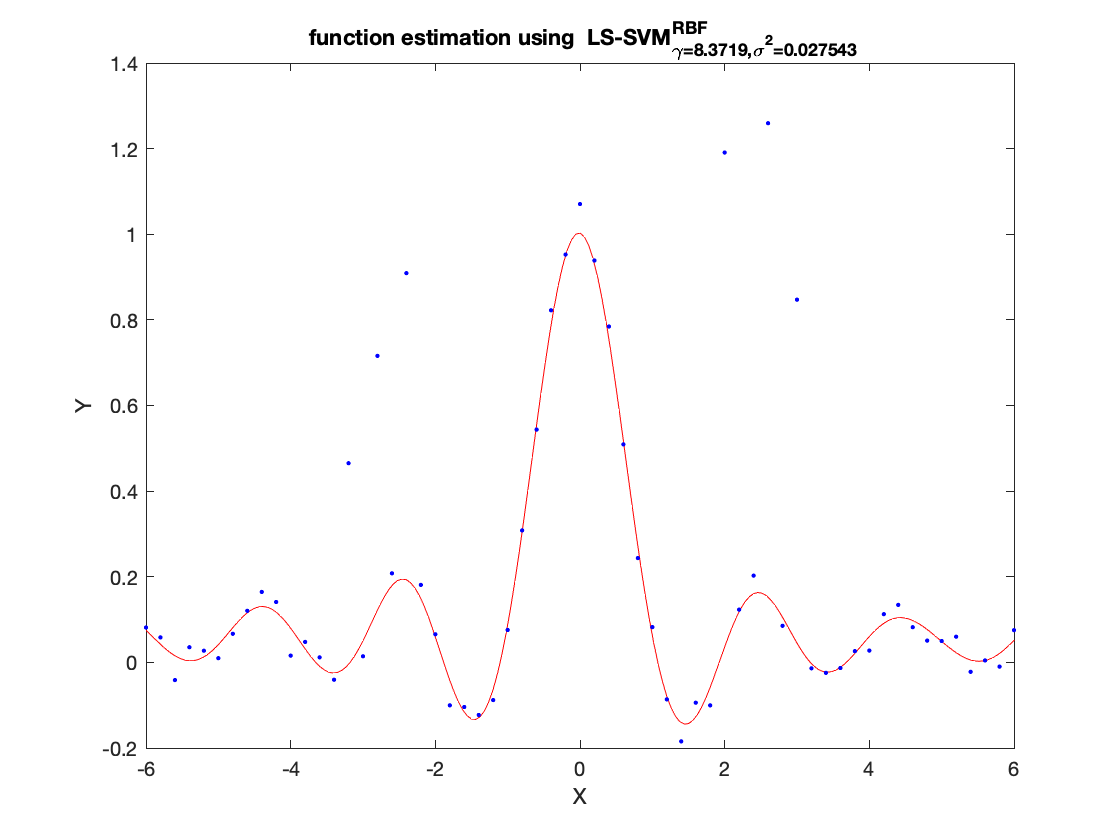
\includegraphics[width=3in]{robustHamper.png}
  \caption{An LS-SVM regression with Hamper weights on the noisy sinc data.}
  \label{fig:hamperRobust}
\end{figure}

\begin{figure}[h!]
\centering
  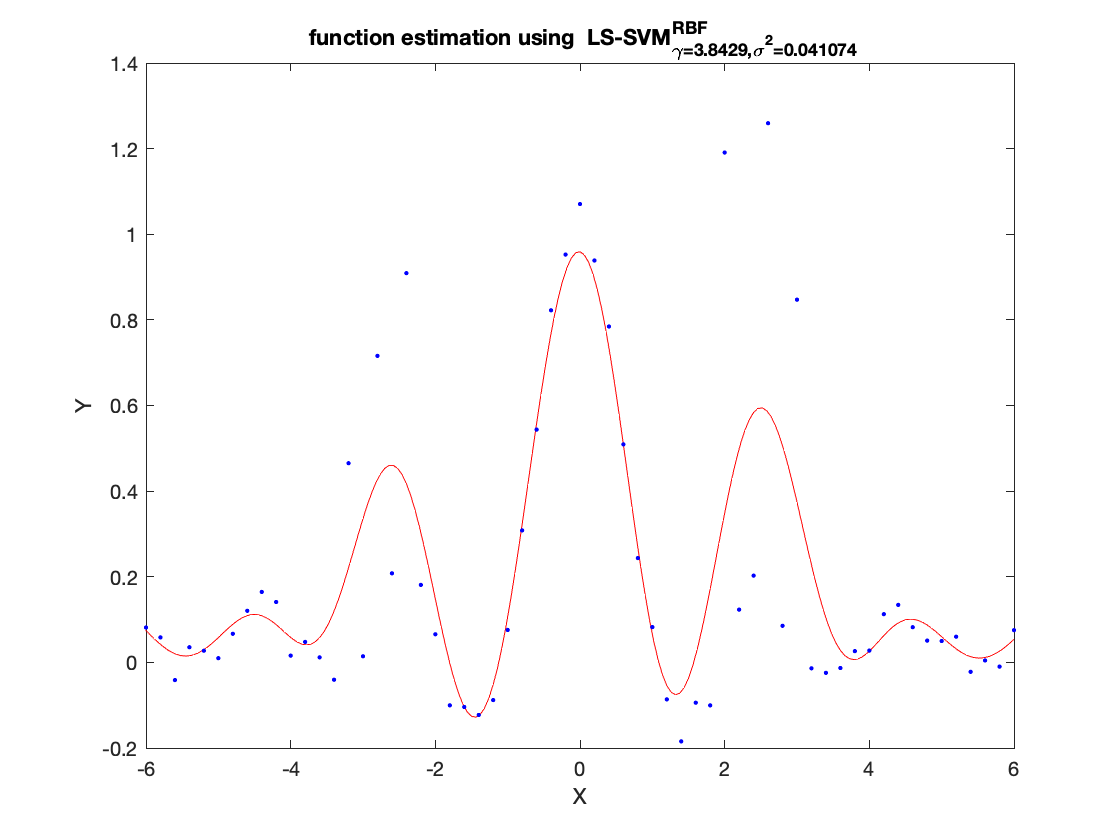
\includegraphics[width=3in]{robustMyriad.png}
  \caption{An LS-SVM regression with myriad weights on the noisy sinc data.}
  \label{fig:myriadRobust}
\end{figure}

\begin{figure}[h!]
\centering
  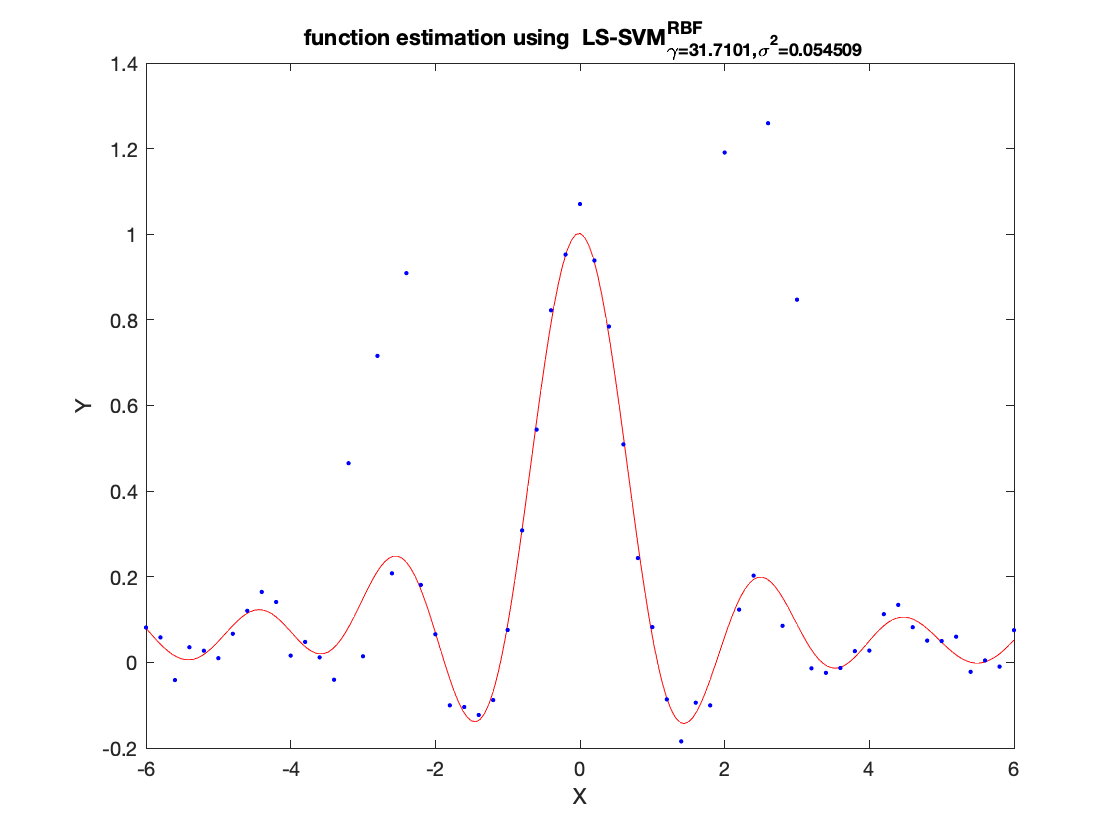
\includegraphics[width=3in]{robustLogistic.png}
  \caption{An LS-SVM regression with Logistic weights on the noisy sinc data.}
  \label{fig:logisticRobust}
\end{figure}



\subsection{Time Series Prediction with Logmap Data}
Time series prediction as done here is nonlinear autoregression exogenous (NARX) modelling. That means that we create a model that uses both the previous values of the dimension of interest and some other, exogenous, variables to predict the future.

This time series dataset contains a number of points in time. The test set is defined to be the points at the last 50 timepoints. After loading the dataset, we can attempt naive prediction of these test points.

\begin{lstlisting}[style=Matlab-editor, frame=single]
order = 10;
X = windowize(Z, 1:(order+1));
Y = X(:, end);
X = X(:, 1:order);
gam = 10; sig = 10;
timeSeriesModel1 = trainlssvm({X, Y, 'f', gam, sig});
Xs = Z(end - order + 1:end, 1);
nb = length(Ztest);
prediction = predict({X, Y, 'f', gam, sig2}, Xs , nb);
\end{lstlisting}

This yields predictions on the test set as depicted in Fig.~\ref{fig:logmapNaive}. Even discounting the fact that time series prediction is notoriously difficult, this is very poor.

\begin{figure}[h!]
\centering
  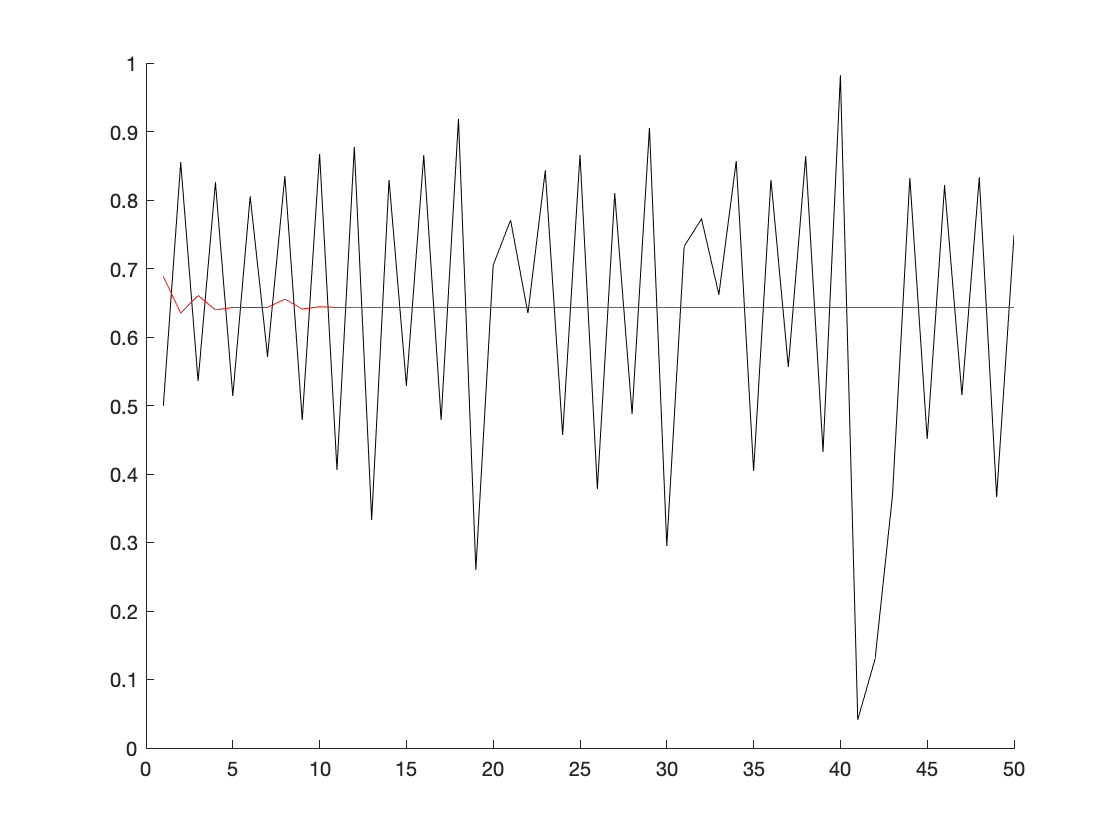
\includegraphics[width=3in]{logmapNaive.png}
  \caption{The result of applying a non-optimised time series prediction model to the logmap dataset, with the test set in black and the predictions in red.}
  \label{fig:logmapNaive}
\end{figure}
 
 Instead, we may use grid search to select a better model. First, use Bayesian inference to select good gam and sig values. Then, we do the grid search.
 
 \begin{lstlisting}[style=Matlab-editor, frame=single]
 gam = 2.4; sig = 24.2154; nb = length(Ztest);
 orderCell = {5 10 20 30 40 50 60 70 80 90 100};
windowizedData = cellfun(@(order) {order, windowize(Z, 1:(order+1))}, orderCell, 'UniformOutput', false);
Yes = cellfun(@(tuple) tuple{2}(:, end), windowizedData, 'UniformOutput', false);
Xes = cellfun(@(tuple) tuple{2}(:, 1:tuple{1}), windowizedData, 'UniformOutput', false);
Xses = cellfun(@(order) Z(end - order + 1:end, 1), orderCell, 'UniformOutput', false);
YandXandXses = arrayfun(@(index) {Yes{index} Xes{index} Xses{index}}, 1:length(orderCell), 'UniformOutput', false);
predictions = cellfun(@(cell) predict({cell{2} , cell{1} , 'f', ...
    gam, sig}, cell{3} ,nb), YandXandXses, 'UniformOutput', false);
   \end{lstlisting}
  
One of the better resulting models is shown in Fig.~\ref{fig:model8Logmap}. Here we see that prediction is very good for some time points and remains relatively poor for others.
   
\begin{figure}[h!]
\centering
  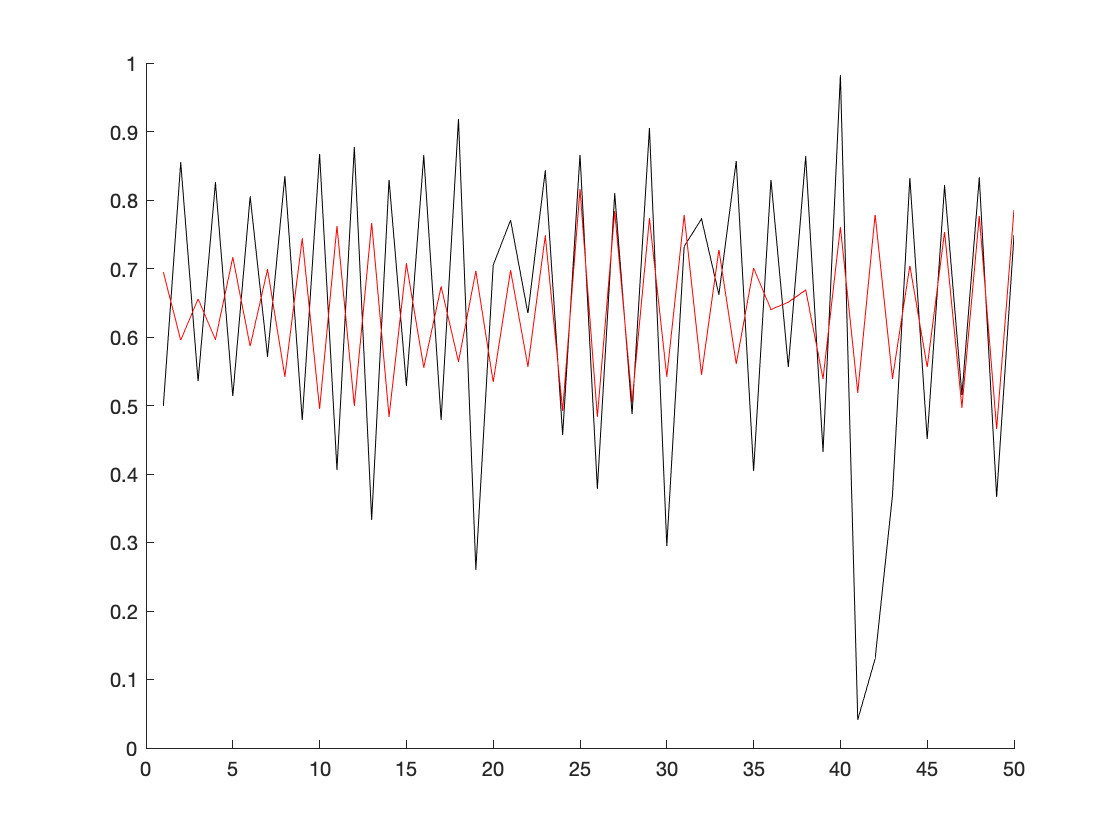
\includegraphics[width=3in]{model8Logmap.png}
  \caption{One of the models resulting from grid search, with the model parameters initially coming from Bayesian inference, with the test set in black and the predictions in red.}
  \label{fig:model8Logmap}
\end{figure}

\subsection{Time Series Prediction with Santa Fe Data}

We may use the same strategy to optimise gam, sig and the order parameters on the Santa Fe dataset. Here a naive fit without optimising parameters results in a bad model. Bayesian inference finds the values $gam=62.47$ and $sig=9.25$ to be good, and we proceed to do grid search as previously, over the same magnitude of orders. At $order=50$, we already have quite good approximation, as can be seen in Fig.~\ref{fig:order50Santa}.

\begin{figure}[h!]
\centering
  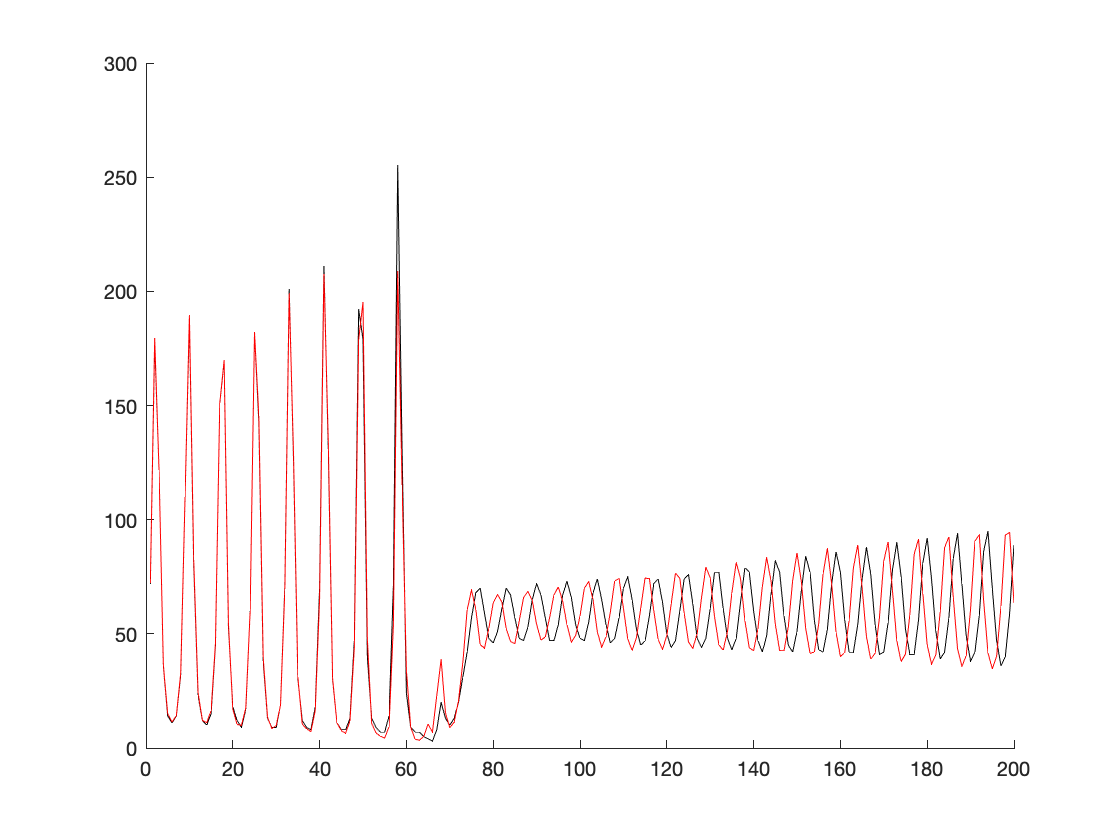
\includegraphics[width=3in]{order50Santa.png}
  \caption{The result of first optimising parameters using Bayesian inference and then doing a grid search of model orders with the Santa Fe dataset, with the test set in black and the predictions in red.}
  \label{fig:order50Santa}
\end{figure}

\bibliographystyle{acm}
\bibliography{SVMbib}
\end{document}